\clearpage{\pagestyle{empty}\cleardoublepage}

\chapter{Testbench}

%\begin{flushright}\begin{small}\textit{"Longum iter est per praecepta, breve et efficax per exempla."}\\
%- Seneca -\\
%\end{small}\end{flushright}

In questo capitolo saranno descritti i testbench realizzati per verificare il corretto funzionamento del componente.

\section{Testbench del componente}

Per testare nello specifico il funzionamento della cache e i meccanismi di comunicazione con la ram, sono stati realizzati 3 file:
 
\begin{itemize}
 \item \texttt{Cache\_test\_ReadAndWrite.vhd}: verifica il corretto funzionamento delle scritture nella cache e nella RAM;
 \item \texttt{Cache\_test\_ReadAndReplacement.vhd}: verifica il corretto funzionamento della politica di rimpiazzamento mediante contatori;
 \item \texttt{Cache\_test\_snoop.vhd}: verifica il corretto funzionamento del protocollo MESI in caso di eventuali snoop.
\end{itemize}

Durante tutti i test eseguiti \`e stata collegata alla cache il componente Ram\_cmp il quale implementa una semplice memoria RAM.\\

Per completezza e per aiutare una successiva lettura delle forme d'onda generate da ISIM durante la simulazione, si riporta fra parentesi dove necessario il valore binario di ci\`o a cui si fa riferimento.

\subsection{Cache\_test\_ReadAndWrite.vhd}
Questo file ha in comune con il resto dei file di testing dei componenti realizzati la dichiarazione dei componenti, il portmap e la fase di reset iniziale. In questo caso specifico il testbench si compone di 3 fasi con le quali si verifica il funzionamento delle scritture:

\subsubsection{Fase 1: Letture d' inizializzazione}
Si caricano in Cache 3 blocchi da 32 byte, 2 in modalit\`a write-back \texttt{ch\_wtwb='0'} e  uno in modalit\`a write-throght \texttt{ch\_wtwb='1'}. Si occupano quindi rispettivamente la via ([x][1]) del primo set di indice ([0][]),  del secondo set di indice ([1][x]) e terzo set di indice ([2][]). In particolare nel terzo set si nota come l'attivazione del segnale \texttt{ch\_wtwb}, porti lo stato (\texttt{.status}) del terzo blocco a 01 ovvero a \texttt{MESI\_S}, mentre negli altri due casi \`e uguale a 10 ovvero \texttt{MESI\_E,} differenza evidenziata in verde nella colonna dei valori nella figura \ref{fig:write1}) .

\begin{figure}[h!]
\centering
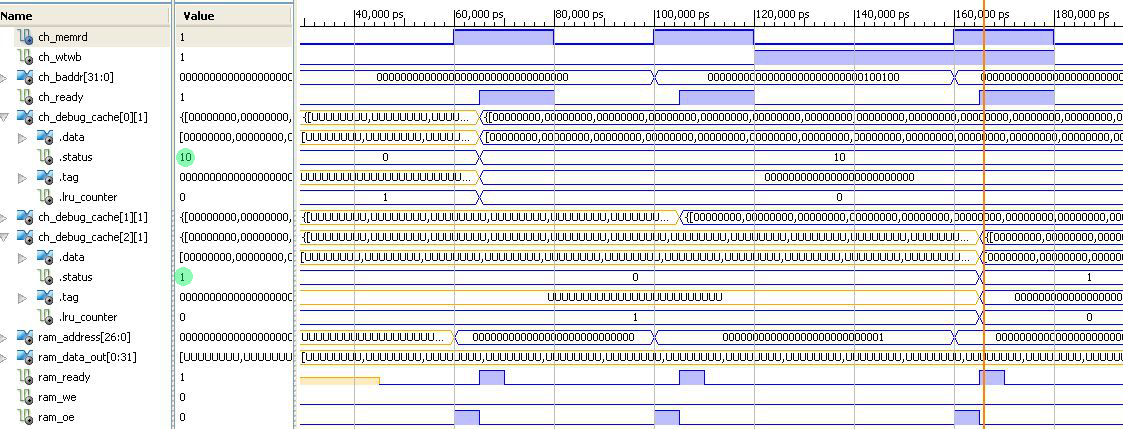
\includegraphics[width=\textwidth]{img/testbench/ReadAndWriteFase1.JPG}
\caption{screenshot ISIM fase 1}
\label{fig:write1}
\end{figure}

\subsubsection{Fase 2: Scritture}
Nella prima scrittura, evidenziata in verde nella figura \ref{fig:write2} avviene un MISS, in quanto il blocco di TAG="10" non \`e ancora presente in cache. Verranno quindi effettuate le seguenti operazioni:
\begin{itemize}
\item lettura in RAM per leggere il blocco contenente il dato e portarlo nella seconda via del primo set ([0][0]);
\item aggiornamento dei valori dei contatori che gestiscono l'invecchiamento per il meccanismo di rimpiazzamento;
\item scrittura in cache aggiornando il valore della word di offset "00110", ovvero i byte dalla posizione [6] alla [9] e lo stato, \texttt{.status} , della via viene posto a MESI\_M ("11").
\end{itemize}
Nella seconda, avviene una scrittura su di un  blocco gi\`a presente in cache, quindi si modifica semplicemente il dato all' offset specificato e si aggiorna lo stato come nel caso precedente.\\
Nella terza scrittura , evidenziata in azzurro nella figura\ref{fig:write2},  a differenza dei due casi precedenti dove la via si porta in stato MESI\_M, la via si porta in MESI\_E inquanto il blocco \`e stato portato in cache in modalita write-throught di conseguenza, la scrittura oltre ad avvenire in cache, avviene anche in RAM, e la nostra cache sar\`a l'unica a possedere il blocco aggiornato, se qualche altro dispositivo possedeva quel blocco, il controllore di memoria dovr\`a preoccuparsi di procedere con l'invalidazione.

\begin{figure}[h!]
\centering
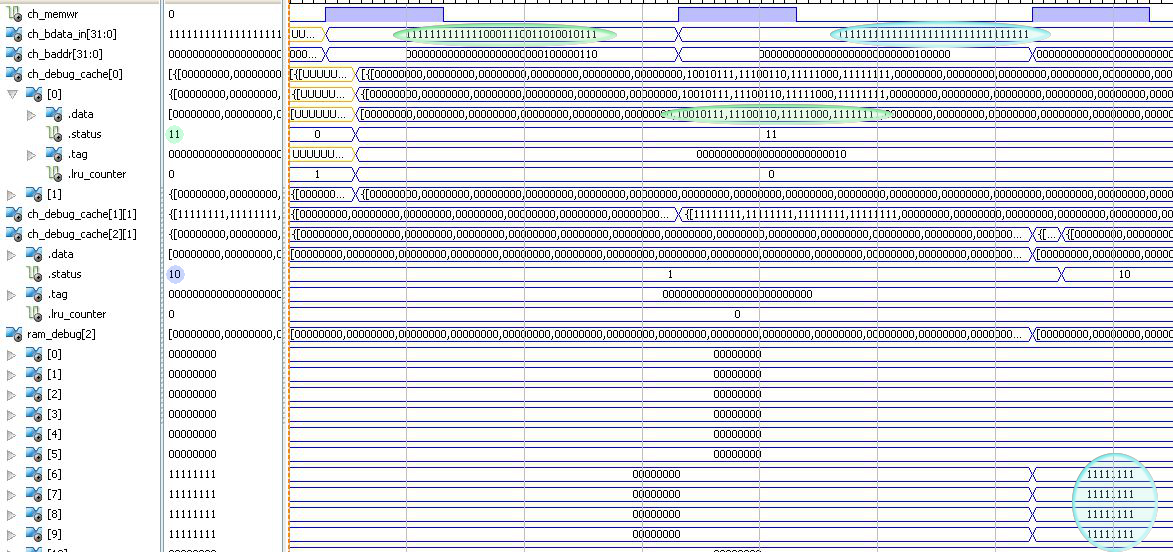
\includegraphics[width=\textwidth]{img/testbench/ReadAndWriteFase2.JPG}
\caption{screenshot ISIM fase 2}
\label{fig:write2}
\end{figure}

\subsubsection{Fase 3: Letture di verifica}
In questa ultima fase vengono eseguite delle letture.
Nel primo caso due letture per verificare i dati scritti nelle prime due scritture.\\
Nel secondo caso(riportato in figura \ref{fig:write3})) si obbliga la cache ad effetture un replacement, in modo da vericare che la cache esegua correttamente il salvataggio in RAM e poi viene ricaricato il blocco originariamente modificato. Consentendoci di verificare immediatamente che il dato che ci viene restituito � quello che era stato originariamente scritto in cache.

\begin{figure}[h!]
\centering
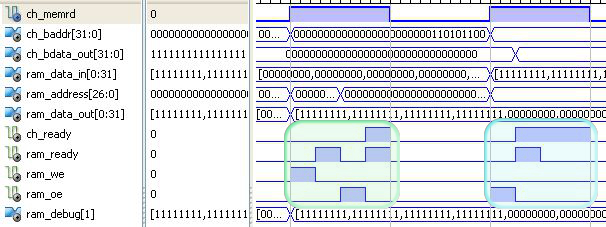
\includegraphics[width=\textwidth]{img/testbench/ReadAndWriteFase3.JPG}
\caption{screenshot ISIM fase 3}
\label{fig:write3}
\end{figure}

Nella figura\ref{fig:write3} si nota inoltre la sequenza di segnali che vengono utilizzati fra RAM e cache per comunicare all'attivazione del segnale \texttt{ch\_memrd}. Nel primo caso, in verde, per scrivere in RAM un blocco modificato presente in cache e nel secondo caso, in azzurro per una lettura in RAM per portare un blocco in cache.

\subsection{Cache\_test\_ReadAndReplacement.vhd}

Questo testbench prevede 3 fasi, con le quali si verifica il corretto funzionamento del meccanismo a contatori per tener traccia di quanto recentemente si \`e acceduti ad una linea di cache, al fine di gestire la politica di rimpiazzamento durante una serie di letture.
Si analizzer\`a infine anche il caso in cui la cache subisca l'invalidazione di una linea.

\subsubsection{Fase 1: Letture di inizializzazione}
Nella prima fase si effettuano 8 letture per riempire tutta la cache.
Avremo quindi tutti i contatori, \texttt{lru\_counter },  delle vie, dei quattro set, che sono stati caricati per ultimi a "0" ,mentre le altre vie avranno il contatore a "1".

\subsubsection{Fase 2: Invalidazione}
Nella seconda fase si esegue un invalidazione sul blocco di TAG="010" e con index="10", ovvero il terzo set; questo comporta il portare lo stato, \texttt{.status}, da MESI\_E(10) a MESI\_I(0) e contatore a "1" nella via che lo contiene mentre l'altra via del set si porta a "0".

\subsubsection{Fase 3: Verifica meccanismo contatori}
Con la prima lettura si verifica che se si effettua una lettura di una word contenuta in un blocco di TAG="0", presente in cache, ovvero abbiamo un hit, il contatore della via([1][1]) dove \`e contenuto viene resettato, mentre le altre vie con valore pi\`u basso di contatore vengono incrementate.\\

Con la seconda lettura si richiede un dato contenuto in un blocco non presente in cache, ovvero abbiamo  miss, viene quindi selezionato il set in base al valore dell' indice, "01" in questo caso e verr\`a rimpiazzato il blocco con valore del contatore pi\`u elevato che in questo caso corrisponde alla via con TAG="10" ( [1][0]) nella quale si era precedentemente resettatato il contatore della via, senza effettuare nessuna scrittura in RAM in quanto il blocco \`e in stato \texttt{MESI\_E}, ovvero il blocco in cache non ha subito nessuna modifica rispetto a quanto presente in RAM.

Con la terza lettura invece si richiede un dato contenuto in un blocco non presente in cache con indice="10", che corrisponde al terzo set ([2][x]), nel quale una via era stata precedentemente invalidata. Tale via([2][0]) verr\`a quindi rimpiazzata senza scrittura in RAM (perch\`e la linea \`e in MESI\_I) con il blocco con TAG="110".

\begin{figure}[h!]
\centering
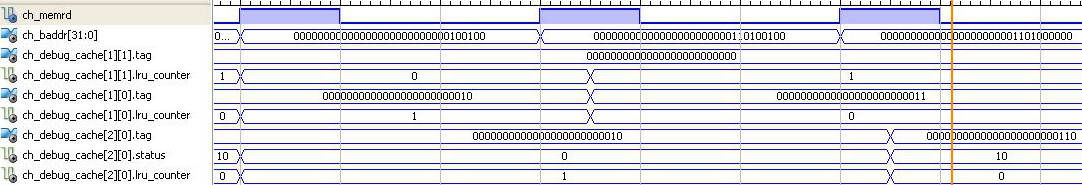
\includegraphics[width=\textwidth]{img/testbench/ReadAndReplacementFase3.JPG}
\caption{screenshot ISIM 3 letture}
\label{fig:replacement3}
\end{figure}

Inifine vengono eseguite una serie di letture su blocchi presenti e non su diversi set e vie, per verificare che tutto nel complesso funzioni correttamente.

\subsection{Cache\_test\_snoop.vhd}
Per prima cosa si inizializza correttamente la cache per permettere di verificare il corretto funzionamento dello snoop nei vari casi. Nello specifico si portano prima in cache due blocchi dalla RAM e sul secondo blocco si esegue una scrittura, per portarlo in stato MESI\_M.\\
In secondo luogo si attiva il segnale di snoop ,\texttt{ch\_eads}, e si imposta l'indirizzo su cui fare lo snoop ,\texttt{ch\_snoop\_addr}. La cache risponder\`a in modo opportuno con i segnali di \texttt{ch\_hit,ch\_hitm} e modificher\`a in alcuni casi lo stato delle vie se il blocco \`e presente in cache.

Nel primo caso si effettua uno snoop su di un blocco che non \`e contenuto in cache, quindi la cache risponder\`a con  \texttt{ch\_hit="0",ch\_hitm="0"}.

Nel secondo caso, evidenziato in giallo in Fig.\ref{fig:snoop1}, si effettua uno snoop su di un blocco presente in cache in stato MESI\_E, quindi la cache risponder\`a con \texttt{ch\_hit="1",ch\_hitm="0"} e porta lo stato della via interessata a MESI\_S("1").

Nel terzo caso, evidenziato in verde in Fig.\ref{fig:snoop1}, si effetua uno snoop su di un blocco che \`e presente in cache in stato MESI\_M("11"). La cache quindi deve:  
\begin{itemize}
\item portare \texttt{ch\_hit="1" e ch\_hitm="1"}
\item forzare la scrittura in RAM del blocco contenuto in cache
\item portare lo stato della via in MESI\_S("1")
\end{itemize}

\begin{figure}[h!]
\centering
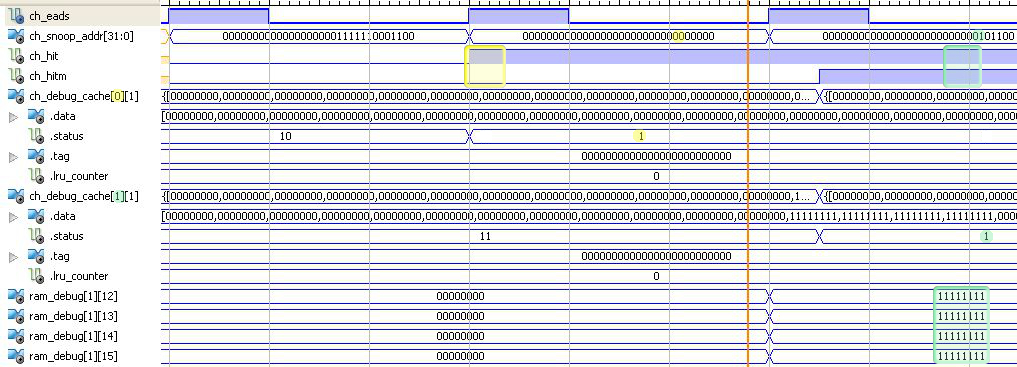
\includegraphics[width=\textwidth]{img/testbench/Snoop1.JPG}
\caption{screenshot ISIM caso 2 e 3 di snoop}
\label{fig:snoop1}
\end{figure}

Infine si effettua una scrittura sul blocco precedentetemente portato in MESI\_S, per verificare che la cache scrivi effetivamente i dati in RAM.

\section{Assembler per DLX}

Dopo avere testato individualmente il funzionamento dei componenti cache e della RAM, si \`e passati al test del corretto funzionamento della cache inserita all'interno del progetto del processore DLX.\\
Per far ci\`o sono stati realizzati una serie di programmi in assembler, dei quali mostreremo solo i due maggiormente significativi:

\begin{itemize}
 \item \texttt{provaReplacement123}: nel quale si verifica la corretta comunicazione tra cache e DLX e il meccanismo di rimpiazzamento.
 \item \texttt{provaFU}: nel quale si verifica il corretto funzionamento della Forwarding unit. 
\end{itemize}

\subsection{Dal codice all'escuzione}
Per completezza in questa sezione si spiegher\`a brevemente come poter mettere in esecuzione un codice assembler.\\
In primo luogo \`e necessario scrivere il codice in assembler all'interno di un file con estensione "*.dls", che viene poi dato in pasto all'assemblatore DASM. Quest'ultimo lo converte in codice macchina mediante il seguente comando, eseguito dal prompt di comandi Windows:\\

\texttt{dasm -a -l <nome\_file>.dls}\\

Il risultato sar\`a un file \texttt{<nome\_file>.dlx} che a sua volta dovr\`a essere convertito mediante la classe java \texttt{DLXConv}, eseguendo dal prompt di comandi Windows:\\

\texttt{java DLXConv <nome\_file>.dlx}\\

 per avere un file  \texttt{<nome\_file>.dlx.txt} contenente il codice in un formato direttamente inseribile all'interno del progetto del DLX.\\

In particolare quest'ultimo dovr\`a essere inserito nel file \texttt{Fetch\_Stage.vhd} all'interno dell'array che rappresenta la EPROM contenente le istruzioni in linguaggio macchina, da dare fare eseguire al processore:\\

\lstset{language=VHDL, caption=Inserimento del codice nella memoria istruzioni, label=DescriptiveLabel, breaklines=true, basicstyle=\small, showspaces=false, showtabs=false, stringstyle=\ttfamily, showstringspaces=false,  tabsize=3} % basicstyle=\tiny\ttfamily}

\begin{lstlisting}

constant EPROM_inst: eprom_type(0 to 11) := ( 
-- istruzioni in linguaggio macchina.
);

\end{lstlisting} 

% \subsection{Codice assembler}
Nei paragrafi successivi si analizzeranno nel dettaglio i codici assembler dei due test pi\`u significativi.
Per comodit\`a si riporter\`a il codice contenuto nella \texttt{EPROM\_inst} corredato di commento e codice assembler relativo.

\subsection{provaReplacement123.vhd}

\lstset{language={[x86masm]Assembler}, caption=Codice assembler per il test del meccanismo di rimpiazzamento, label=DescriptiveLabel, breaklines=true, basicstyle=\footnotesize\ttfamily, showspaces=false, showtabs=false, showstringspaces=false,  tabsize=3} % basicstyle=\tiny\ttfamily}

\begin{lstlisting}
X"20010000",	--l1: addi r1,r0,0 ; azzera r1
X"20020001",	--l2: addi r2,r0,1 ; imposta a 1 r2
X"AC220000",	--l3: sw 0(r1),r2 ; memorizzza il valore di r2 all'indirizzo 0+r1(via 1 dell index0)
X"20420001",	--l4: addi r2,r2,1 ; incrementa r2
X"AC220100",	--l5: sw 16#100(r1),r2 ; memorizzza il valore di r2 all'indirizzo 16#100+r1(via 0 dell index0)
X"20420001",	--l6: addi r2,r2,1 ; incrementa r2
X"AC220080",	--l7: sw 16#80(r1),r2 ; memorizzza il valore di r2 all'indirizzo 16#80+r1(replacement via 1 dell index0) 
X"8C220000",	--l8: lw r2,0(r1) ; ripristina valore iniziale di r2 (1)
X"20210004",	--l9: addi r1,r1,4 ; incremento di 4 indirizzo di base in r1
X"0BFFFFE0",	--l10: j l3 ;
X"FFFFFFFF",	--NOP 
X"FFFFFFFF" 	--NOP

\end{lstlisting} 
Questo codice conta fino a tre, da qui il nome del file termina con 123, ad ogni iterazione ricomincia da uno, inoltre ogni risultato intermedio viene salvato in memoria in una locazione diversa in modo da obbligare la cache, ad ogni iterazione, a rimpiazzare un blocco, lavorando sempre nel primo set, per un  numero limitato d'iterazioni. Infatti, ad esempio nella prima iterazione, quando r1="0",si nota che i due bit che identificano l'indice sono sempre uguali a "00":\\

\begin{itemize}
  \item l3) \texttt{0(r1)=0+0= "000 00 00000"} ovvero prima via occupata nel primo set ( [0][1] ) siccome  b6=0 e b7=0;
  \item l5) \texttt{16\#100(r1)="010 00 00000"} ovvero seconda via occupata nel primo set( [0][0] );
  \item l7) \texttt{16\#80(r1)= "001 00 00000"} ovvero prima via rimpiazzata nel primo set( [0][1] ), quindi si ha una scrittura in RAM del blocco modificato seguita da una lettura del nuovo blocco.
\end{itemize}


Si continuer\`a a operare nel primo set finch\`e il valore di r1 non supera trentuno, ovvero alla trentaduesima iterazione si passer\`a a lavorare sul secondo set, ma questo non avverr\`a mai nella nostra simulazione, data la durata limitata del testbench.\\

In seguito si effettua il caricamento in r2 del primo valore scritto in memoria (ovvero "1"), ma il blocco che contiene la word di indirizzo 0 non \`e pi\`u presente in cache, verra quindi effettuato un ulteriore rimpiazzamento per� sulla seconda via([0]).\\
Infine si incrementa in valore di r1 di quattro unit\`a in modo da scrivere non pi\`u nel byte di offset "00000" ma di offset "00010", ovvero la word successiva di ogni blocco.\\

\begin{figure}[h!]
\centering
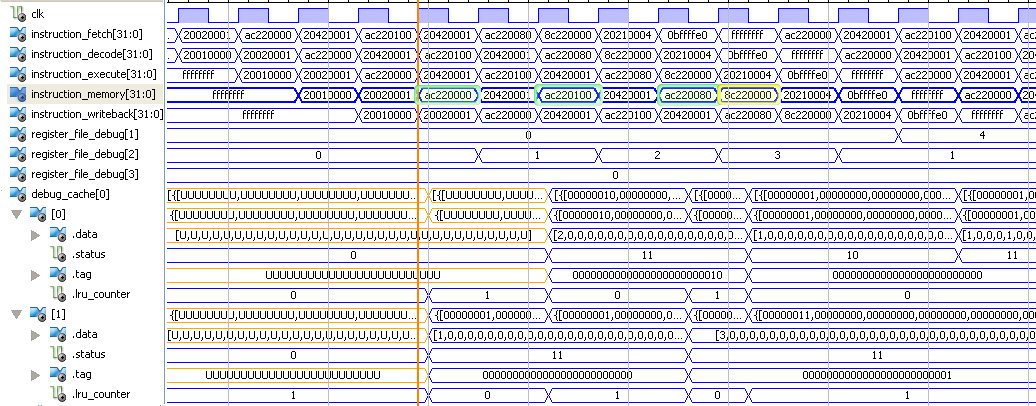
\includegraphics[width=\textwidth]{img/testbench/DLX123.JPG}
\caption{evidenziato in verde le store e in giallo le load}
\label{fig:DLX123}
\end{figure}

\subsection{provaFU.vhd}
In questo programma si testa il corretto funzionamento della Forwarding Unit per evitare un alea di dato.\\
Il codice da sostituire all'interno del \texttt{EPROM\_inst}, al posto di quello dell'esempio precedente, \`e il seguente:\\

\lstset{language={[x86masm]Assembler}, caption=Codice assembler per il test della Forwarding Unit, label=DescriptiveLabel, breaklines=true, basicstyle=\footnotesize\ttfamily, showspaces=false, showtabs=false, showstringspaces=false,  tabsize=3} % basicstyle=\tiny\ttfamily}

\begin{lstlisting}
X"20420001",  --l1: addi r2,r2,1  ; porta a 1 il valore di r2
X"AC220000",  --l2: sw 0(r1),r2  ; salva il contenuto di r2
X"8C230000",  --l3: lw r3,0(r1)  ; porta in r3 il valore presente in r2
X"20620001",  --l4: addi r2,r3,1  ; incrementa r2
X"0BFFFFF0",  --l5: j l2          ; salta a l1
X"FFFFFFFF",  --NOP

\end{lstlisting} 

La Forwarding Unit viene sfruttata nel quinto ciclo di clock per evitare un'alea si dato di tipo RAW. Si nota che l'istruzione \texttt{X"20620001"} nello stadio di EX vuole leggere il valore contenuto in r3 per incrementarlo di uno ma \`e appena stato caricato dalla cache dall'istruzione (lw r3,0(r1)) presente nello stadio di MEM, pertanto il dato non � ancora disponibile nel Register File e vi sarebbe un'alea di dato. Per far fronte a ci\`o, la Forwarding Unit fornir\`a il dato presente nello stadio di MEM attraverso i segnali \texttt{mem\_dest\_register} e \texttt{mem\_dest\_register\_data} allo stadio di EXE.\\

\begin{figure}[h!]
\centering
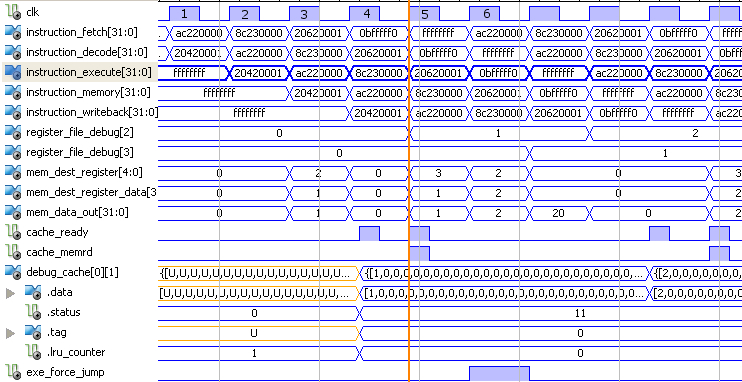
\includegraphics[width=\textwidth]{img/testbench/DLXFU.JPG}
\caption{Screenshot ISIM di provaFU}
\label{fig:DLXFU}
\end{figure}

Nella Fig. \ref{fig:DLXFU} sono mostrati:
\begin{itemize}
   \item l'istruzione critica in giallo;
   \item i valori forniti dalla Forwarding Unit e il risultato corretto in verde;
   \item i valori  non aggiornati forniti dallo stadio di decode in rosso.
\end{itemize}
